% Inside the generation stage: text path, image paths, flow model, decode.
% Render: pdflatex -interaction=nonstopmode diagram_generation_internals.tex
% Then:  pdftoppm -png -r 400 -singlefile diagram_generation_internals.pdf out
% The picture is exactly \textwidth wide, so the deck places it with width=\linewidth.
\documentclass[border=0pt,11pt]{standalone}
\usepackage[T1]{fontenc}
\usepackage[utf8]{inputenc}
\usepackage{helvet}
\renewcommand{\familydefault}{\sfdefault}
\usepackage{tikz}
\usetikzlibrary{positioning,arrows.meta}

\definecolor{primaryNavy}{RGB}{24,24,27}
\definecolor{secondaryNavy}{RGB}{63,63,70}
\definecolor{mutedGray}{RGB}{248,250,252}
\definecolor{ruleGray}{RGB}{226,232,240}

% main label, then a smaller second line
\newcommand{\twoline}[2]{#1\\[1.5pt]{\footnotesize\color{secondaryNavy}#2}}

\tikzset{
  proc/.style={draw=secondaryNavy,line width=0.5pt,fill=mutedGray,text=primaryNavy,
               font=\small,align=center,inner xsep=4pt,inner ysep=3.5pt,
               minimum height=0.62cm,minimum width=2.25cm},
  data/.style={text=primaryNavy,font=\small,align=center,inner sep=1.5pt},
  feed/.style={draw=secondaryNavy,line width=0.6pt},
  fl/.style={draw=secondaryNavy,line width=0.6pt,
             -{Stealth[length=1.7mm,width=1.4mm]}},
}

\begin{document}
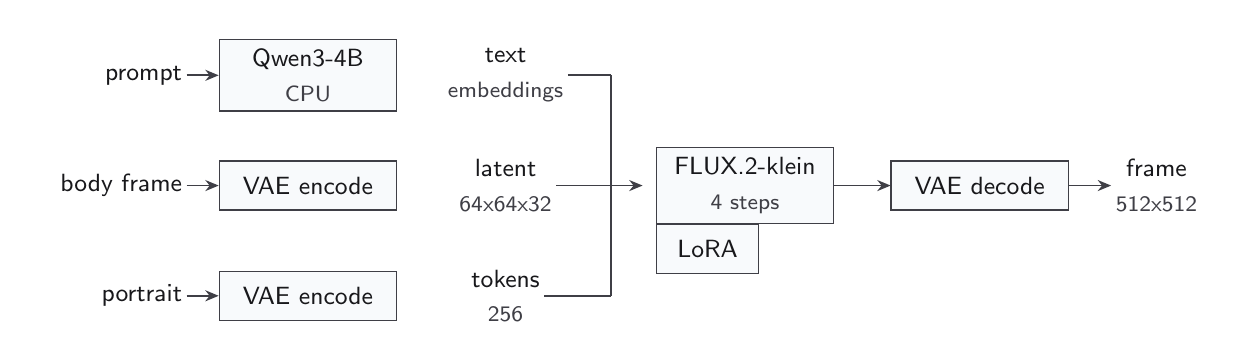
\begin{tikzpicture}
\useasboundingbox (0.2303cm,-2.2151cm) rectangle (0.2303cm+433.34402pt,1.6552cm);
\fill[white] (0.2303cm,-2.2151cm) rectangle (0.2303cm+433.34402pt,1.6552cm);

% ---- top row: the conditioning path ----------------------------------------
\node[data,anchor=east] (pr) at (2.25,1.05) {prompt};
\node[proc] (qwen) at (3.79,1.05) {\twoline{Qwen3-4B}{CPU}};
\node[data] (te) at (6.30,1.05) {\twoline{text}{embeddings}};

% ---- image paths -----------------------------------------------------------
\node[data,anchor=east] (bf) at (2.25,-0.35) {body frame};
\node[proc] (vae1) at (3.79,-0.35) {VAE encode};
\node[data] (lat) at (6.30,-0.35) {\twoline{latent}{64x64x32}};

\node[data,anchor=east] (po) at (2.25,-1.75) {portrait};
\node[proc] (vae2) at (3.79,-1.75) {VAE encode};
\node[data] (tok) at (6.30,-1.75) {\twoline{tokens}{256}};

% ---- inputs into the flow model --------------------------------------------
\draw[fl] (pr) -- (qwen);
\draw[fl] (bf) -- (vae1);
\draw[fl] (po) -- (vae2);

% ---- the bundle of embeddings and latents feeds the flow model -------------
\draw[feed] (te.east) -- (7.64,1.05);
\draw[feed] (lat.east) -- (7.64,-0.35);
\draw[feed] (tok.east) -- (7.64,-1.75);
\draw[feed] (7.64,1.05) -- (7.64,-1.75);
\draw[fl] (7.64,-0.35) -- (8.04,-0.35);

% ---- flow model with its adapter -------------------------------------------
\node[proc] (flux) at (9.34,-0.35) {\twoline{FLUX.2-klein}{4 steps}};
\node[proc,minimum width=1.3cm,anchor=north west] (lora) at (flux.south west) {LoRA};

% ---- decode ----------------------------------------------------------------
\draw[fl] (flux.east) -- (11.19,-0.35);
\node[proc] (vdec) at (12.32,-0.35) {VAE decode};
\node[data,anchor=west] (out) at (13.99,-0.35) {\twoline{frame}{512x512}};
\draw[fl] (vdec.east) -- (out.west);
\end{tikzpicture}
\end{document}
